% This file was converted to LaTeX by Writer2LaTeX ver. 1.4
% see http://writer2latex.sourceforge.net for more info
\documentclass[a4paper, 12pt]{article}
\usepackage[utf8]{inputenc}

\usepackage[T1]{fontenc}
\usepackage{times}
%\usepackage[T1]{fontenc}
%\usepackage{lmodern}
\usepackage[english]{babel}
\usepackage{amsmath}
\usepackage{amssymb,amsfonts,textcomp}
\usepackage{array}
\usepackage{hhline}
\usepackage[pdftex]{graphicx}
\usepackage[hidelinks]{hyperref} % to hide ugly links use
\def\UrlBreaks{\do\/\do-} % To break urls at the end of the line

% For bibliography:
\usepackage[
%    natbib = true,
%     backend=bibtex, % this OR biber
backend=biber,
isbn=false,
url=false,
doi=false,
eprint=false,
%    style=numeric,
%style=authoryear,
style=authoryear-comp,
sorting=ynt, % sorts names in citations by year, name, then title
sortcites = true, % to avoid first names, but check disambiguation in the very end:
uniquename=false,
uniquelist=false,
maxbibnames=3,    
maxcitenames=2 % to put "et al" after a few authors
]{biblatex}
\renewcommand*{\nameyeardelim}{\space} % to remove the coma in textcite (bug work around)
\bibliography{bibzotero}
% To clear the "note" field:
\AtEveryBibitem{%
	\clearfield{note}%
}
\AtEveryBibitem{%
	\clearlist{language}%
}

\emergencystretch 2em % To avoide overfull boxes
\renewcommand{\baselinestretch}{1.5}

%\topskip=40pt
%\parskip=10pt
%\parindent=0pt
%\baselineskip=15pt

\usepackage{geometry}
\geometry{a4paper, portrait, left=2.5cm, right=2.5cm}
%%\textwidth=12.978986403cm % golden ratio
%%\addtolength{\oddsidemargin}{1cm}
%%\addtolength{\evensidemargin}{1cm}
%%%\addtolength{\textwidth}{-2cm}
\addtolength{\topmargin}{-0.5cm}
\addtolength{\textheight}{1.5cm}

\title{\Huge Mate-copying in Drosophila:\\ a matter of taste or disgust?}
\author{Guillaume Lespagnol}
\date{\today}

\begin{document}
	
	\maketitle
	
	\tableofcontents
	
	\bigskip
%	\clearpage
	
%	Examples of citation: \textcite[e.g.][118]{danchin_cultural_2018}.
	
%	Or rather:
	\parencite[118]{danchin_cultural_2018}.

%	\parencite{}
	Or several: \textcites[e.g.][118]{danchin_cultural_2018}[but see][1789]{danchin_cultural_2018}

	\parencite{}
%	Or several: \textcites[e.g.][118]{danchin_cultural_2018}[but see][1789]{pike_conformist_2010}

	
	Or between brackets: \parencites{danchin_cultural_2018}[but see][1789]{dagaeff_drosophila_2016}.
	
%	\parencite{framit_zotero_2019, morgan_biological_2012}.
	
%	\textcite{dagaeff_drosophila_2016} demonstrated that...
	
	\section{Introduction}






	Sexual selection is at the origin of an intense struggle between conspecifics. In some species, it is by harm and winning is a matter of weight, strength or weapons \parencite{anderson_grey_1985, clutton-brock_functions_1982}. In others it is by charms in a much more peaceful contest, and the breeders are chosen by the other sex.
	The mate-choice (i.e intersexual selection) can lead to captivating and highly complex traits, such as courtships or songs in birds \parencite{danchin_ecologie_2005}. Nevertheless, many species do not exhibit such traits and the choice is based on much more ambiguous and discreet signs.
	“The most difficult and important act of choice is the choice of a mate” \parencite{fisher_evolution_1915}, in context of mate-choice making a mistake can be very expensive since it impact individual’s offspring.
	To avoid mistakes, many species have acquired the capacity to learn from the observation of others and can therefore use social learning in numerous decision-making processes.
	
	Social learning can take different form, as teaching or copying. The latter is simpler, and even exists in non-social invertebrates\parencite{coolen_social_2005,laidre_mark_e._how_2010}. 
	Many different behaviours can be copied \parencite{thornton_alex_multi-generational_2010, van_leeuwen_group-specific_2014}.
	 It’s particularly beneficial when individual learning is costly (time consuming or dangerous; also see \parencite{webster_m.m_social_2008}) as in mate-choice.
	 Therefore, copying the mate-choice of potentially older conspecifics can be a reliable choice for naive individuals to avoid unnecessary mistakes.
	
	
	Mate-copying is a form of social learning in which the observation of a sexual interaction between conspecifics biases the subsequent mate-choice decision of the observer \parencite{brown_fish_2011}.
	It has been first demonstrated in fishes \parencite{dugatkin_lee_alan_reversal_1992}, followed by observations in many vertebrates \parencite{galef_mate-choice_1998, yorzinski_same-sex_2010} and recently in invertebrates \parencite{mery_public_2009, fowler-finn_complexities_2015}.
	Its benefits are  double-sided, it allows naive individuals to avoid mistakes and make sure that their descendants will be preferred by conspecifics. 
	Interestingly, in population with genetic preferences, mate-copying can override them \parencite{dugatkin_interface_1996, witte_male_1998}.
	At larger  scale, mate-copying can even shape preferences of entire populations and potentially lead to formation of local traditions.
	Such traditions transmitted vertically and horizontally for a trait-based preference and possibly for a long time can even lead to the appearance of  animal culture\parencite{brooks_importance_1998, danchin_cultural_2018}.
	
	The existence of culture in non-human species has long been disputed \parencite{laland_animals_2003} but is increasingly accepted among scientists \parencite{aplin_experimentally_2015, whitehead_geneculture_2017}. 
	The list of animals exhibiting a form of cultural tradition is growing constantly \parencite{van_schaik_orangutan_2003, thornton_alex_multi-generational_2010, whiten_culture_2017} , and one of the most recent may surprise many, Drosophila melanogaster \parencite{danchin_cultural_2018}. 
	Very few, if none, species have been studied as deeply and for whom knowledge in every scientific field (genetics, development, neuroscience…) is as extensive than Drosophila Melanogaster. 
	Thus existence of mate-copying in this species represents a wondeful opportunity to understand the obscure neuronal root of an evolutive behavior broadly shared in the animal kingdom.
	
	In drosophila, depending on if the stimulus is aversive or appetitive, different groups of neurons are involved \parencite{vogt_shared_2014,busto_olfactory_2010}. 
	Therefore, our first step was to test if mate-copying implies aversive or appetitive memory, by isolating different kinds of stimulus contained in copulation of conspecifics. 
	We considered that a rejection represent an aversive stimulus and acceptance of copulation an appetitive stimulus for an observer female. 
	So, we created two treatments by presenting a male rejected by a female ("Rejection" treatment) or a male accepted by a female ("Acceptance" treatment), for which we measured the inclination to copy. 
	
	Then we investigated deeper neuronal mechanisms of mate-copying by searching which group of neurons is required for mate-copying. 
	Indeed, the neuronal mechanisms of non-social learning is very well known in Drosophila (reviewed in \textcite{cognigni_right_2018}).
	Regarding their roles in the latter, two brain structures are particularly prone to be involved in mate-copying, the central complex and the mushroom body.
	The central complex, localized in the center of the insect brain plays a major role in decoding visual information.
	It receives visual inputs from the rest of the brain and controls vision-related behaviors, memory and learning \parencite{guo_vision_2017}.
	The mushroom body is an integrative center involved in learning, memory, decision-making  and visual associative memory.
	Notably, specific groups of dopaminergic neurons localized in mushroom bodies are involved in the acquisition of aversive and appetitive visual  memory \parencite{liu_subset_2012, vogt_shared_2014}. 
	On the contrary, despite a rich repertoire of well-studied social processes \parencite{pasquaretta_how_2016, teseo_fighting_2016, dawson_social_2018}, neuronal mechanisms of social learning are still poorly understood. 
	However, a recent study have found that dopamine is required in mate-copying \parencite{monier_dopamine_2018}.
	Dopamine is a neurotransmitter, that drive a  variety of brain function among which the formation of appetitive and aversive memory \parencite{riemensperger_punishment_2005,sitaraman_serotonin_2008,alekseyenko_targeted_2010,berry_dopamine_2012,yamamoto_dopamine_2014}. Dopamine is produced in dopaminergic neurons but we do not know which are involved in mate-copying. 
	However, we do know some of the neurons required for non-social visual memory.
	\textcite{vogt_shared_2014} showed that neurons labeled by TH-GAL4 and Ddc-GAL4 transgene are essential in visual learning. 
	Given that mate-copying involves visual learning, we expect these neurons to be required.
	Thanks to Liu et al., we know that UAS-GAL4 technology can be used to block specific sets of neurons \parencite{liu_subset_2012}. Precisely, by coupling UAS-GAL4 with the Shibire protein, it is possible to temporary silence specific groups of neurons and investigate in what processes they are essential. 
	Our goal was to use a similar technique but concerning mate-copying. We used mutant flies expressing GAL4 in TH-labeled or Ddc-labeled neurons, that we have silenced to see if those neurons are required in mate-copying (for more details, see "Fly stains and crossings" section). 
	We thus created two treatments: ``Th'' and ``DDC'' depending of the group of the neurons silenced, for which we calculated mate-copying scores. 
	If one group is involved in mate-copying, the corresponding treatment will exhibit a mate-copying score similar to random choice, due to the incapacity of mutants to learn.
	
	
	\section{Material and Methods}

	\subsection{Fly maintenance}
	
	We used the common Canton-S strain of D.melanogaster (wild-type, and UAS / Gal4 lines described above). Flies were raised and kept in 30 ml tubes containing standard corn flour-yeast-agar medium at 25° ± 1°C and 56 ± 4 \% humidity with a 12:12H light:dark cycle. Humidity and temperature were controlled and adjusted continuously with two independents automatic humidifiers and one manual heater. Medium was cooked every 3 weeks and stored at 4°C until use. Flies were manipulated with a hand-made mouth aspirator made of a glass pipette, tubing and gauze.
	
	Every morning, adult flies were removed from the breeding vials so that the newly emerged flies collected within the 6-8 hours were virgin. For Canton-S strain, 120 males and 120 females were used daily for breeding (20 tubes with 6 males and 6 females in each) and all other adults were euthanized in a freezer. For mutant strains, all adults were used for breeding. 
	
	Virgins were sexed without anesthesia, by gentle aspiration and then kept in unisex groups of 7 females or 14 males until experiments. Both demonstrator and observer flies were 3 or 4 days old. Males and females were used only once as females are reluctant to re-mate \parencite{chapman_sex_2003} and reject males they just saw copulating \parencite{loyau_when_2012}. After experiments, all flies were put in a food vial and cold-euthanized at the end of the day.
	
	\subsection{Fly stains and crossings}
	
	For the second experiment, we used two mutant genotypes, Ddc-GAL4/w+;;UAS-Shits/+ and w+/w-;;UAS-Shits/TH-GAL4 ,obtained by crossing homozygous lines. 
	
	UAS-Shits is a transgene that contains an GAL4-specific enhancer,UAS (Upstream Activating Sequence) driving the production of Shibire protein in cells where GAL4 is present. Shibire is a thermosensitive protein that inhibit neuronal activity at restrictive temperature (30°C) by preventing vesicle recycling \parencite{kitamoto_conditional_2001}. Ddc-GAL4 and TH-GAL4 drive production of a transcriptional activator (GAL4) only in specific subsets of dopaminergic neurons. GAL4 activates the expression of genes downstream to UAS. Ddc-GAL4 labels neurons involved in appetitive olfactory memory:the blockade of these neurons by Shibire protein has been shown to impair the acquisition of such memory at restrictive temperature.TH-GAL4 labels neurons involved in aversive olfactory memory \parencite{liu_subset_2012}.
	
	As white recessive mutation w- impairs fly vision \parencite{gotz_optomotorische_1964}, we used mutant females with one wild-type copy of the white gene for the experiments. To do so, we crossed w+;;Shits males with females from each Gal4 line. To obtain w+;;Shits strain from a w-;;Shits strain, we crossed males w-;;Shits with females w+;;TM2/TM6b over two generations and selected TM2 non TM6B flies only, with CO2 anesthesia, and we then isolated homozygous w+;;Shits progeny.
	
	TH-GAL4 and Ddc-GAL4 lines were provided by Guillaume Isabel in the same Canton-S background as the Wild-type strain.
	
	\subsection{General experimental procedures}
	
	Artificial male phenotypes were created by dusting virgin males with pink or green powder \parencite{mery_public_2009}. Each vial of males was randomly assigned to a color. Before the experiment started, males were placed in a clean vial to remove the excess of dust for at least 20-30 min. Experiments took place in the same tube set-up and a similar but slightly modified speed-learning protocol than described in \textcite{dagaeff_drosophila_2016} (Figure 1, see also specific experiment section).
	
	Demonstrator and observer flies were placed in two compartments of double plastic tubes, separated by a thin glass partition and closed by cotton plugs. All replicates were run in blocks of six trials with cardboard barriers between experimental set-ups, to prevent information exchange between the flies and disturbance from the surroundings. 
	
	During the demonstration, we always showed two different male phenotypes (color) to the observer females, with one favorite that copulated with the demonstrator female. If demonstrator females refused to copulate, the trial was discarded. Specifics of demonstrations for each experiment are described above (see specific experiment section).
	
	Once the demonstrations were over, we started the mate-copying test by introducing a couple of colored virgin males (one of each color) in front of the observer female and we removed the partition, allowing the female to freely choose between males for 30 min. The partition was put back in place when all three flies were in the same side of the tubes, to promote proximity between flies. During that time, we recorded the time of first courtship for each male, the time when copulation started and the color of the chosen male. The onset of the courtship was defined as the first wing-extension of a male (Figure 2).

	\begin{figure}
	\centering
	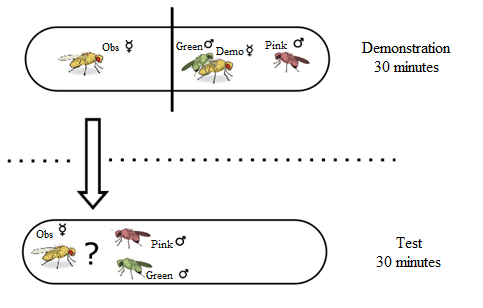
\includegraphics[width=0.6\textwidth]{images/classic}
	\caption{Légende ici.}
	\label{fig:Classic protocol}
	\end{figure}

	\subsubsection{Acceptance/Rejection experiment}
	
	During this first experiment, we tested whether mate-copying is achieved through aversive or appetitive memory. To do so, we split the negative and positive information given by the usual mate-copying demonstration. A classical demonstration, in which a demonstrator female chooses between two males, contains a rejection (negative information) of a male and an acceptance (positive information) of the other one. We thus created three demonstration treatments: (1) a control where a demonstrator female freely chooses between two males, (2) an “acceptance” treatment with one accepted male copulating with a demonstrator female, and (3) a rejection treatment with one male actively rejected by a female (Figure 3).
	
	\subsubsection{Neuronal blockade experiment}
	
	This second experiment aimed at exploring the mechanisms underlying the results of the Acceptance/Rejection experiment by discovering one group of dopaminergic neurons involved in mate-copying.
	
	The demonstration was similar to classical protocol (Figure 1), but we used Ddc-GAL4/w+;;UAS-Shits/+ (treatment “Ddc”) and w+/w-;;UAS-Shits/TH-GAL4 mutants (treatment “Gal4”) as observer females. The use of these mutants allowed us to have a temporal control on specific sets of neurons presumably involved in appetitive (Ddc) or aversive (TH) memory, thanks to the thermosensitive activation of Shibire. During the demonstration and 30 minutes before, observer mutant females were heated to a restrictive temperature of 33°C, thanks to a heating mat under the tube of these females. At 33°C, Shibire protein blocks the neurons in which it is expressed, and thus the acquisition of appetitive memory should be blocked in observer females of “Ddc” treatment, and the acquisition of aversive memory in “TH” females. 
	
	After all copulations ended, demonstrator males and females were removed. Observer females were then stored individually in clean tubes at 25°C for 3-4 hours to ensure that labelled neurons are no more blocked, then we proceeded to a classical test at 25°C.

	\begin{figure}
	\centering
	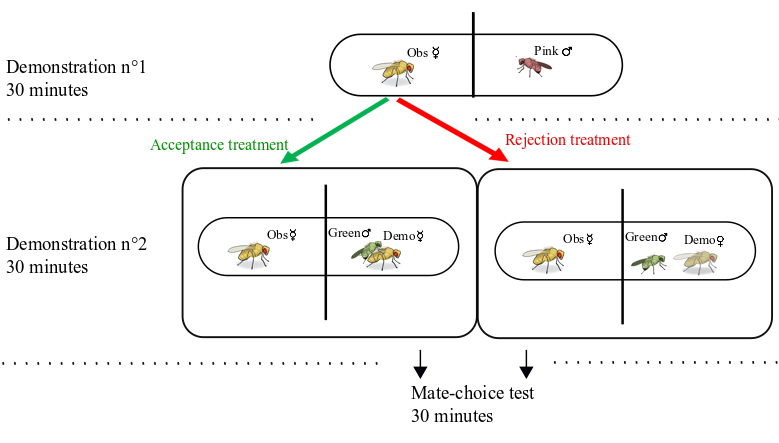
\includegraphics[width=0.8\textwidth]{images/ar}
	\caption{Légende ici.}
	\label{fig:ar}
\end{figure}

	\subsection{Mate-copying score}

	As in previous studies \parencite{danchin_cultural_2018,nobel_mate-copying_2018,monier_dopamine_2018}, a mate-copying score evaluated female’s tendency to copy the choice of the demonstrator. A mate-copying score of 1 was assigned to females that copulated with the color preferred by demonstrator females and a score of 0 in the opposite case. For each treatment, a mate-copying index was calculated as the mean of mate-copying scores per treatment, a random choice indicated by a value of 0.5. All replicates where only one male courted the female before copulation were discarded because in these situations the female was not unambiguously in a position to make a choice between the two colors.

	\subsection{Statistical analyses}

	All statistical analyses were performed with the R software version 3.5.1 (R Core Team, 2018).
	For each treatment, the difference from a random choice was tested with a binomial test. Mate-copying scores were then analyzed in a generalized linear mixed model (GLMM, package lme4 \parencite{bates_fitting_2015}). Starting models contained the following fixed effects: treatment, normalized air pressure (air pressure in Toulouse-Blagnac weather station, at the time of the beginning of the experiment, minus mean air pressure), normalized air pressure variation within the six preceding hours and all interaction between these three variables, experimenter effect and its interaction with treatment. A random “block” effect was also introduced in the models to account for the non-independence of observer flies from the same block of 6 tubes-set up trained and tested in parallel. The significance of fixed effects was tested using Wald chi-square tests included in ANOVA function (car package, \textcite{fox_r_2018} ). Model simplification was achieved by successive withdrawal of the non-significant terms in a backward selection approach, using P-values and starting with the highest-order interaction. The final model was chosen as the one with the lowest Akaike Information Criteria (AIC, Akaike, 1969). Comparisons between treatments were done using post-hoc X² tests. 

	\subsection{Ethical statements}

	Behavioral observations of D. melanogaster required no ethical approval and complied with French laws regarding animal welfare. We kept the number of flies used in this study as small as possible. We handled flies by gentle aspiration without anesthesia to minimize damage and discomfort. After the experiments, individuals were euthanized in a freezer at -20°C.

	\section{Results}

	\subsection{A/R Experiment}
	\label{subsec:AR-experiment}

	For this experiment, we tested 850 females among which 530 copulated during test, including 192 with double-courtship, 64 for each treatment. First we tested for female's color preference with binomial test but neither in the demonstration (N = 850, 426 females copulated with green males and 424 copulated with pink males; binomial test: P = 0.973) nor the test (N = 530, 270 copulated with green and 260 with pink males; binomial test: P = 0.696) was there any significant difference between the two colors.

	For each treatment, the difference from random choice was tested with a binomial test, ``acceptance'' (where the observer female sees a copulation, N = 64, P {\textless} 0.001) and ``control'' (N = 64, P = 0.03) were both significantly different from random, but ``rejection'' treatment (where the observer female sees a male rejected without copulation, N = 64, P = 0.382) was not (Figure 4).

	To test for the significance of mate copying among treatments, we built a global model including the effects of experimenter, treatment, normalized air pressure (actual air pressure minus global mean of air pressure), normalized air pressure variation (for the last six hours) and the interaction between air pressure and variation of air pressure. The selected model included the effect of treatment, air pressure, variation of air pressure and the interaction between air pressure and its variation. Only the treatment had a significant effect on mate-copying (GLMM, $\chi^2$: $N = 192$, $\chi^2 = 10.447$, $p = 0.005$), air pressure (GLMM, $\chi $²: N = 192, $\chi $² = 0.572, p = 0.449) and variation of air pressure (GLMM $\chi $²: N = 192, $\chi $² = 1.831, p = 0.176) were non-significant. The interaction between air pressure and variation of air pressure was close to be significant (GLMM $\chi $²: N = 192, $\chi $² = 2.946, p = 0.086), as we could have expected in regard of the results of \textcite{dagaeff_drosophila_2016}. No significant difference has been found between ``control'' and ``acceptance'' treatments ($\chi $² = 1.76, P = 0.18; Fig4), but both are different from ``rejection'' treatment (acceptance - rejection: $\chi $² = 11.62, P {\textless} 0.005; control - rejection: $\chi $² = 4.52, P = 0.033; Fig4).
	
\subsection{Neuronal blockade experiment}

For this second experiment, we tested 336 females, among which 208 copulated, including 88 with double courtship. Female's color preference was tested with a binomial test, but we found no preference between the two colors in demonstrations (N = 336, 151 females copulated with green males and 185 copulated with pink males; binomial test: p {\textless}0.072) and tests (N = 208, 107 copulated with green and 101 with pink males; binomial test: p {\textless}0.729).
As for the previous experiment, we first tested difference from random choice for each treatment with a binomial test: females from ``Ddc'' treatment exhibited a mate-copying score different from random (N = 39, p {\textless} 0.024) while ``TH'' did not (N = 49, p {\textless} 0.568)(Fig 5).
To test for the effect of treatment on mate-copying efficiency, we built a global model, including the effects of experimenter, treatment, normalized air pressure (actual air pressure minus global mean of air pressure), normalized air pressure variation (for the last six hours) and the interaction between air pressure and variation of air pressure. The selected model included the effect of treatment, air pressure, variation of air pressure and the interaction between air pressure and its variation.Again, only the treatment had a significant effect on mate-copying (GLMM, $\chi^2$: $N = 88$, $\chi^2 = 4.245$, $p = 0.0394$), while effect of air pressure, variation of air pressure and interaction between air pressure and air pressure variation were non-significant (GLMM, $\chi^2$: $N = 88$, $\chi^2$ = $0.619$, $0.259$ and $2.176$ respectively, $p = 0.4315$, $0.611$ and $0.14$ respectively)(Fig 4).
	Voir Figure~(\ref{fig:mcsar}).
		\begin{figure}
		\centering
		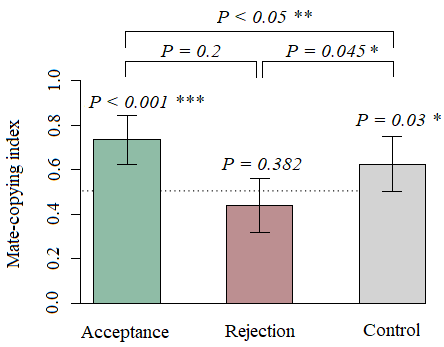
\includegraphics[width=0.8\textwidth]{images/mcsar}
		\caption{Légende ici.}
		\label{fig:mcsar}
	\end{figure}


\section{Discussion}

So far, mate-copying studies in \textit{Drosophila melanogaster} were based on the acceptance or rejection of different phenotypes by a demonstrator.
Here we showed that the acceptance, not the rejection, of a single male is sufficient to induce mate-copying in females. 
When a female witnessed an acceptance of male followed by a copulation, she exhibited mate-copying. 
In the other case, when observer female witnessed only a rejection of the male, her subsequent choices was similar to random. 
In both cases, only a part of the information was available for the female; but it seems that negative information is not used, since mate-copying score are not significantly different between control and rejection. 
Although several studies have already demonstrated mate-copying without copulation between demonstrators in fish, they are hardly comparable to our study. 
As it was not about copulation but time spent close to the favorite male \parencite{dugatkin_lee_alan_reversal_1992,galef_mate-choice_1998}. 
Notably, a study on lekking birds (\textit{Terao tetrix})  showed that females exhibited mate-copying only when the males were able to copulate with demonstrator females. 
But again, mate-copying was not a matter of biased copulation but of biased attraction to preferred males. 
In our study, both demonstration and test involved copulation and so it leave little doubt about results. 
The fact that mate-copying relies on acceptance and positive information rather than rejection and negative information is pertinent in regard of evolution.
Females can reject copulation for several individual-specific reasons and so acceptance is much more informative.
For example, in flies a female can reject a male if she recently mated \parencite{chapman_sex_2003}. 
In this case, the reason for rejection is pointless for other females and uninformative about the male quality, which is potentially excellent. 
Whereas for acceptance, the quality of the male is more likely to play a role in it.
%Nevertheless, the mate-choice is based on many factors, and acceptance is not always relevant as a source of information observers.
%so?
However, we used non-virgin demonstrator females in rejection experiment, and males can smell that the female has recently mated \parencite{jallon_few_1984}. Even though we made sure the male courted the female, it is possible that his behaviors differs and that the female observer sees it. In these conditions, its inclination to copy the choice of demonstrator may be impacted, leading to the observed results. This point demand further investigation.




%	Voir Figure~(\ref{fig:mcsar}).
 
%	\begin{figure}
%		\centering
%		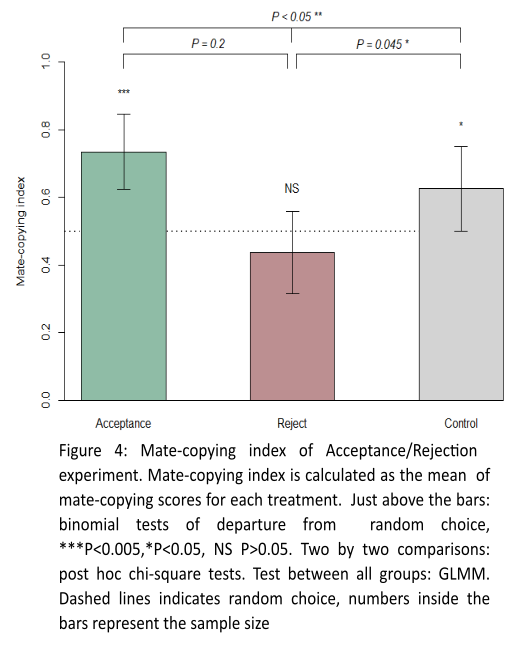
\includegraphics[width=0.8\textwidth]{images/histogramme-mcs}
%		\caption{Légende ici.}
%		\label{fig:histogramme-mcs}
%	\end{figure}





\clearpage
\newrefcontext[sorting=nyt] % sorts the bibliography by name first, then year, title
\printbibliography
 \end{document}
